\documentclass[french]{book}

\usepackage[top=2cm, bottom=2cm, left=2cm, right=2cm]{geometry}

\usepackage[T1]{fontenc}
\usepackage[utf8]{inputenc}
\usepackage{babel}
\usepackage{pdflscape}
\usepackage{titlesec}
\usepackage{multicol}
\usepackage[inline]{enumitem}
\usepackage{amsmath, amsthm, amssymb}
\usepackage{mathrsfs}
\usepackage{float}
\usepackage{caption}
\usepackage{hyperref} % Liens dans la table des matières


% TikZ

\usepackage{tikz}
\usetikzlibrary{babel}
\usetikzlibrary{calc}
\usetikzlibrary{arrows}
\usetikzlibrary{patterns}
\usetikzlibrary{decorations.pathmorphing, decorations.markings}
\usetikzlibrary{positioning}
\usetikzlibrary{optics}


% "north east hatch" pattern
\makeatletter
\tikzset{% customization of pattern 
        hatch distance/.store in=\hatchdistance,
        hatch distance=5pt,
        hatch thickness/.store in=\hatchthickness,
        hatch thickness=5pt
        }
\pgfdeclarepatternformonly[\hatchdistance,\hatchthickness]{north east hatch}% name
    {\pgfqpoint{-1pt}{-1pt}}% below left
    {\pgfqpoint{\hatchdistance}{\hatchdistance}}% above right
    {\pgfpoint{\hatchdistance-1pt}{\hatchdistance-1pt}}%
    {
        \pgfsetcolor{\tikz@pattern@color}
        \pgfsetlinewidth{\hatchthickness}
        \pgfpathmoveto{\pgfqpoint{0pt}{0pt}}
        \pgfpathlineto{\pgfqpoint{\hatchdistance}{\hatchdistance}}
        \pgfusepath{stroke}
    }
\makeatother

\tikzset{>=stealth}
\tikzset{schema/.style={rounded corners=#1, fill=lightgray, draw, inner sep=0pt},
         schema/.default=4pt}
\tikzset{bati/.style={pattern=north east hatch, hatch distance=7pt, hatch thickness=1.2pt, preaction={fill=lightgray}}}
\tikzset{ressort/.style 2 args={decorate, decoration={coil,aspect=#1,segment length=#2,amplitude=3mm}}}


% Pour les spectres d'émission / d'absorption

\usepackage{pgf-spectra}


% Couverture

\ifpdf
	\usepackage{pdfcolmk}
\fi

\ifxetex
	\usepackage{fontspec}
\fi

\usepackage{url}
\usepackage{graphicx}
\usepackage{pifont}

\newlength{\drop}

\newcommand*{\mytitle}{\begin{titlepage}
\begingroup
\drop = 0.13\textheight
\centering
\vspace*{\drop}
{\Huge Physique (\textsc{mpsi})}\\[\baselineskip]
{\Huge\itshape Année scolaire 2017-2018}\\[3\baselineskip]
{\Large \textit{Cours de} \textsc{N. Tancrez}}\par
\vfill
{\begin{center}\includegraphics[scale=1.5]{SL.png}\end{center}}
\vspace*{1cm}
{\Large Lycée Saint-Louis}\par
\vspace*{\drop}
\endgroup
\end{titlepage}}



% Style des sections

\titleformat{\chapter}
[frame] % format
{\vspace*{5cm}\Huge} % format du texte
{\thechapter} % format du label
{1cm} % séparation
{\centering\sffamily} % avant
[\thispagestyle{empty}] % après


% pour la table des matières
\titleformat{name=\chapter, numberless}
[display] % format
{\Large\bfseries} % format du texte
{\titlerule} % format du label
{-7ex} % séparation
{\centering\MakeUppercase} % avant


\titleformat{\section}
[block] % format
{\LARGE\bfseries} % format du texte
{\thesection} % format du label
{8pt} % séparation
{\centering} % avant

\titleformat*{\subsection}{\Large\bfseries}


\renewcommand{\thechapter}{\Roman{chapter}}
\renewcommand{\thesection}{\arabic{section}.}
\renewcommand{\thesubsection}{\Roman{subsection}}

\pagestyle{plain} % Numéro de page en bas de la page
\setcounter{tocdepth}{1} % On ne veut que les sections

% Math environments

\newtheorem*{lemme}{Lemme}
\newtheorem*{theoreme}{Théorème}
\newtheorem*{propriete}{Propriété}

\theoremstyle{definition}
\newtheorem*{definition}{Définition}
\newtheorem*{exemple}{Exemple}
\newtheorem*{exemples}{Exemples}
\newtheorem*{experience}{Expérience}
\newtheorem*{vocabulaire}{Vocabulaire}

\theoremstyle{remark}
\newtheorem*{remarque}{Remarque}


% Math macros

\usepackage{mathtools}

\DeclarePairedDelimiter\abs{\lvert}{\rvert}
 
\makeatletter
\let\oldabs\abs
\def\abs{\@ifstar{\oldabs}{\oldabs*}}
\makeatother


\newcommand*\dif{\mathop{}\!\mathrm{d}}


% Conventions du cours

\newcommand*{\point}[1]{\mathrm{#1}}
\newcommand*{\systeme}[1]{\mathrm{#1}}
\newcommand*{\vecteur}[1]{\overrightarrow{#1}}
\newcommand*{\algebrique}[1]{#1'}


\newcommand*{\tdef}[1]{\textbf{#1}}
\newcommand*{\imp}[1]{\emph{#1}}
\newcommand*{\abr}[1]{\textsc{#1}}



% Où chercher les fichiers

\makeatletter
\def\input@path{{01_signaux_harmoniques_propagation/}, {02_optique_geometrique/}}
\makeatother

\newcommand{\cours}[2]
{\begin{landscape}
\begin{multicols*}{2}[\section{#1}]
\input{#2}
\end{multicols*}
\end{landscape}}


%%%%%%% Document %%%%%%%

\begin{document}

% Titre

\mytitle

\tableofcontents

\chapter{\textsc{Signaux harmoniques et propagation}}

\cours{Oscillateur harmonique}{01_oscillateur_harmonique}
\cours{Propagation d'un signal}{02_propagation_signal}
\cours{Ondes progressives sinusoïdales}{03_ondes_progressives_sinusoidales}
\cours{Interférences}{04_interferences}
\cours{Ondes stationnaires}{05_ondes_stationnaires}
\cours{Diffraction}{06_diffraction}

% TODO : ordres de grandeur

\chapter{\textsc{Optique géométrique}}

\cours{Description ondulatoire de la lumière}{01_description_ondulatoire_lumiere}
\cours{Modèle géométrique de la lumière}{02_modele_geometrique_lumiere}
\cours{Systèmes optiques}{03_systemes_optiques}



\begin{landscape}
\begin{multicols*}{2}[\section{Formation des images}]

\subsection{Systèmes centrés}

\begin{definition}
Un \imp{système optique} est \tdef{centré} s'il possède un axe de révolution, alors appelé \tdef{axe optique}.
\end{definition}

\begin{definition}
Un \imp{système centré} est \tdef{rigoureusement aplanétique} si l'image $\point{A'}\point{B'}$ de tout objet $\point{A}\point{B}$ plan et perpendiculaire à son axe optique l'est aussi.

\begin{figure}[H]
\begin{center}
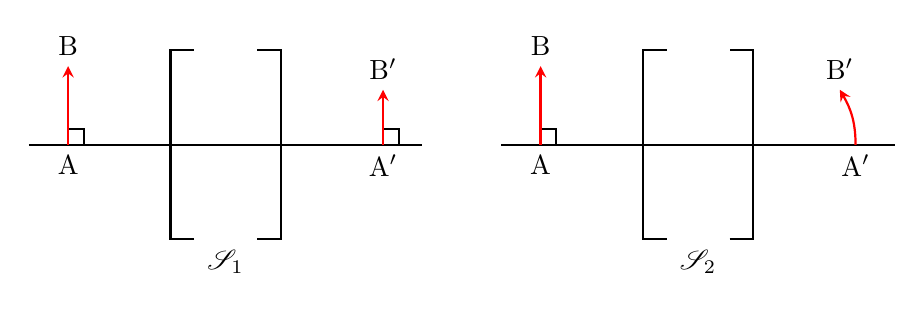
\begin{tikzpicture}[thick, use optics]
\coordinate (O1)  at (-3,0);
\coordinate (O2)  at (3,0);
\coordinate (A)   at (-2,0);
\coordinate (B)   at (-2,1);
\coordinate (A')  at (2,0);
\coordinate (B'1) at (2,0.7);
\coordinate (B'2) at (1.8,0.7);

% Système 1

\draw (O1) +(-2.5,0) -- +(2.5,0);

\draw ($ (O1) + (A) + (0,0.2) $)  -| ($ (O1) + (A) + (0.2,0) $);
\draw ($ (O1) + (A') + (0,0.2) $) -| ($ (O1) + (A') + (0.2,0) $);

\draw [red, ->] ($ (O1) + (A) $)  -- ($ (O1) + (B) $);
\draw [red, ->] ($ (O1) + (A') $) -- ($ (O1) + (B'1) $);
\node [below] at ($ (O1) + (A) $)   {$\point{A}$};
\node [above] at ($ (O1) + (B) $)   {$\point{B}$};
\node [below] at ($ (O1) + (A') $)  {$\point{A'}$};
\node [above] at ($ (O1) + (B'1) $) {$\point{B'}$};

\draw (O1) +(-0.4,-1.2) -- +(-0.7,-1.2) -- +(-0.7,1.2) -- +(-0.4,1.2);
\draw  (O1) +(0.4,-1.2) -- +(0.7,-1.2)  -- +(0.7,1.2)  -- +(0.4,1.2);
\node [below] at ($ (O1) + (0,-1.2) $) {$\mathscr{S}_1$};


% Système 2

\draw (O2) +(-2.5,0) -- +(2.5,0);

\draw ($ (O2) + (A) + (0,0.2) $) -| ($ (O2) + (A) + (0.2,0) $);

\draw [red, ->] ($ (O2) + (A) $)  -- ($ (O2) + (B) $);
\draw [red, ->, out=90, in=-60] ($ (O2) + (A') $) to ($ (O2) + (B'2) $);
\node [below] at ($ (O2) + (A) $)   {$\point{A}$};
\node [above] at ($ (O2) + (B) $)   {$\point{B}$};
\node [below] at ($ (O2) + (A') $)  {$\point{A'}$};
\node [above] at ($ (O2) + (B'2) $) {$\point{B'}$};

\draw (O2) +(-0.4,-1.2) -- +(-0.7,-1.2) -- +(-0.7,1.2) -- +(-0.4,1.2);
\draw  (O2) +(0.4,-1.2) -- +(0.7,-1.2)  -- +(0.7,1.2)  -- +(0.4,1.2);
\node [below] at ($ (O2) + (0,-1.2) $) {$\mathscr{S}_2$};
\end{tikzpicture}
\end{center}

\captionsetup{labelformat=empty}
\caption{Le système optique $\mathscr{S}_1$ est aplanétique, contrairement à $\mathscr{S}_2$}

\end{figure}
\end{definition}



\subsection{Conditions de Gauss}

\begin{definition}
Les \tdef{conditions de Gauss} pour un \imp{système centré} consiste à n'utiliser que des \tdef{rayons paraxiaux}, c'est-à-dire proches de l'axe optique et peu inclinés par rapport à celui-ci.
\end{definition}

\begin{remarque}
On se place en pratique dans les \imp{conditions de Gauss} en \imp{diaphragmant} le système et en observant des objets petits ou éloignés :

\begin{figure}[H]
\begin{center}
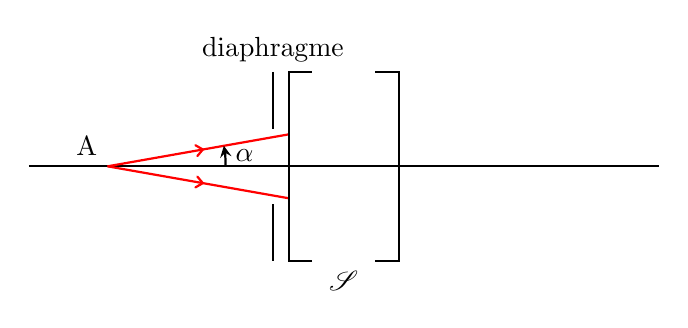
\begin{tikzpicture}[thick, use optics]
\coordinate (A) at (-3,0);

\node [diaphragm, object height=2.4cm] (diaphragme) at (-0.9,0) {};
\node [above] at (diaphragme.north) {diaphragme};

\draw (-4,0) -- (4,0);

\node [above left] at (A) {$\point{A}$};
\draw [red, ->-] (A) -- +(10:2.34);
\draw [red, ->-] (A) -- +(-10:2.34);
\draw [->] (A) +(1.5,0) arc (0:10:1.5) node [midway, right] {$\alpha$};

\draw (-0.4,-1.2) -- (-0.7,-1.2) -- (-0.7,1.2) -- (-0.4,1.2);
\draw  (0.4,-1.2) --  (0.7,-1.2) --  (0.7,1.2) --  (0.4,1.2);
\node [below] at (0,-1.2) {$\mathscr{S}$};
\end{tikzpicture}
\end{center}
\end{figure}
\end{remarque}

\begin{definition}
L'\tdef{approximation de Gauss} (ou \tdef{approximation des petits angles}) consiste à confondre fonctions trigonométriques et approximation affine :

\begin{center}
\begin{itemize*}[itemjoin=\qquad]
\item $\cos \alpha \simeq 1$
\item $\sin \alpha \simeq \alpha$ (mais $\sin^2 \alpha \simeq \alpha^2 \simeq 0$)
\item $\tan \alpha \simeq \alpha$
\end{itemize*}
\end{center}
\end{definition}

\begin{propriete}
Les \imp{conditions de Gauss} permettent d'obtenir un stigmatisme et un aplanétisme approché, et d'utiliser l'approximation de Gauss.
\end{propriete}



\subsection{Foyers et plans focaux}

\begin{definition}
Un \tdef{objet ponctuel à l'infini} (resp. \tdef{image ponctuelle à l'infini}) est un faisceau de \imp{rayons incidents} (resp. \imp{émergents}) parallèles, que l'on repère à l'aide de son inclinaison par rapport à l'axe optique.
\end{definition}

\begin{definition}
Le \tdef{foyer objet} $\point{F}$ (resp. \tdef{foyer image} $\point{F'}$) est le point objet dont l'image se trouve à l'infini sur l'axe optique.
\end{definition}


\end{multicols*}
\end{landscape}

\end{document}
